\chapter{Introduction}\label{ch:introduction}
\setlength{\epigraphwidth}{3in}
\epigraph{Three can keep a secret, if two of them are dead.}{Benjamin
  Franklin}

This book is about finding and exposing data that are \emph{hidden},
\emph{invisible}, or simply \emph{overlooked} in digital systems. When
such data that are privacy sensitive are discovered, the results
frequently include pain, ruined
reputations, financial loss, and even harms to national
security. 

\section{Leaks of Private Information \DONE}

Consider these three cases:

\begin{itemize}
\item Today's smart phones use a combination of signals from Global
  Positioning System (GPS) satellites and terrestrial Wi-Fi access
  points to determine their position. In April 2011, two software
  developers discovered that Apple's iOS~4 operating system kept an
  on-phone database of every Wi-Fi access point and its GPS location
  that the phone had ever encountered. The purpose of this database
  was to allow the phone to rapidly determine where it was without
  having to use the GPS receiver. Unfortunately, the database was
  never purged, and it was copied to the user's laptop or desktop
  computer whenever the iPhone was backed up using Apple's
  \emph{iTunes} program\cite{apple-tracking}. To demonstrate the
  privacy leak, the developers created an application exported the
  data and plot it with Google Maps~(\figref{heatmap}). A media uproar
  resulted, forcing Apple to make an unplanned release of its
  operating system that fixed the bug\cite{apple-tracking-statement}.

\item The Portable Document Format (PDF) used by Adobe Acrobat was
  designed to make it easy for organizations to publish printed
  documents as electronic files. But unlike printed files, electronic
  documents can contain information that's present but doesn't
  print---information that is effectively invisible. Such data can
  cause significant problems for individuals, organizations and even
  governments. That's what happened in April 2011 when the UK
  Parliament posted an Adobe Acrobat file on its public with sensitive
  military information about UK nuclear subs. Although the file had
  been redacted and cleared by the British Ministry of Defense (MOD),
  \emph{The Daily Telegraph} discovered that the information had
  merely been covered with black boxes, rather than being actually
  removed.\label{uk-mod} A follow-up investigation found other PDF
  files that had improperly redacted on four other UK government
  websites\cite{telegraph-april2011-secrets}.

\item Sometimes even software that promises to delete information
  somehow doesn't. That's what the Utah-based company Decipher
  Forensics discovered in May 2013 when it analyzed cell phones that
  had been used with the popular \emph{Snapchat} application, which
  lets users send photos with an expiration date. What the Decipher
  Forensics discovered was that even 
  though Snapchat was promising users that it deleted the photos, in
  fact they were only hidden and could still be recovered with
  digital forensic tools\cite{ksl-snap-chat}.

\end{itemize}

\begin{figure}
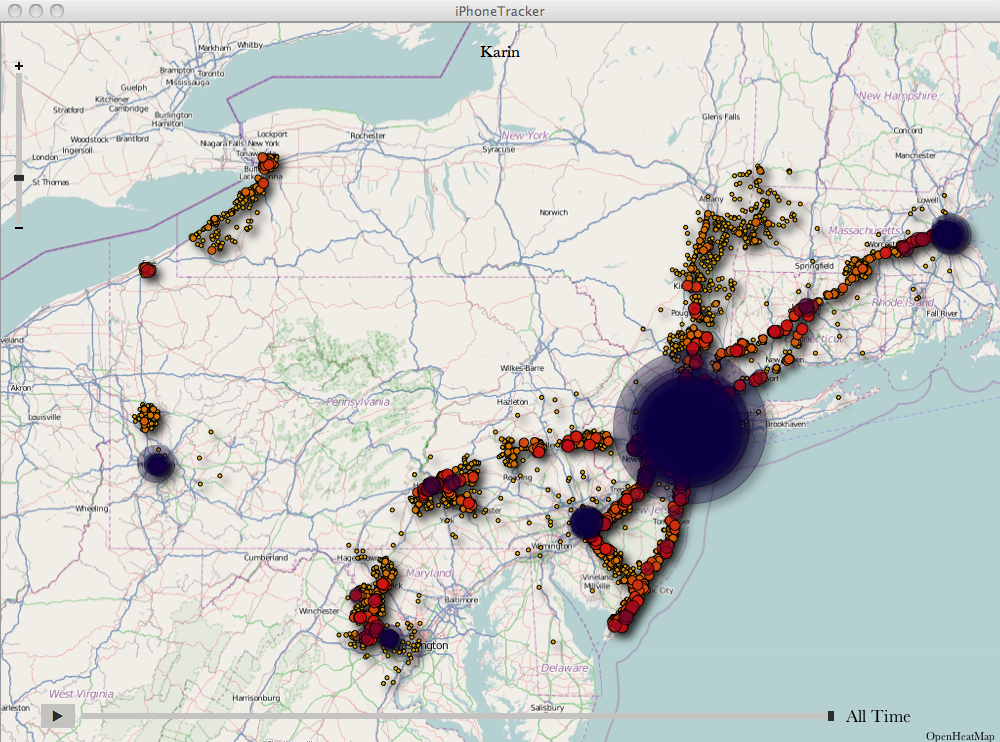
\includegraphics[width=\textwidth]{ch-1/5637893141_ba59f2d989_o.png}
\caption{In April 2011, Pete Warden and Alasdair Allan discovered
that Apple's iOS~4
  operating system recorded the location of nearby Wi-Fi access points
  to aid in geolocation. Due to a bug the database was never
  cleaned. As a result, the database could easily be used to create a
  map of every place that the iPhone had been. \rights{\copyright 2011 John
  Niedermeyer. Licensed under Creative Commons
  Attribution-NonCommercial-ShareAlike 2.0 Generic.}}\label{heatmap}
% http://www.flickr.com/photos/nedward/5637893141
\end{figure}

Hidden data are present in many computer systems. They are stored in
documents, embedded in operating systems, and even encoded and sent over
networks. It's not the \emph{presence} of these data that damages
privacy---it's their inevitable discovery and exploitation.

Most of the technical privacy failures that we know about were not
discovered by the companies that wrote the software in
question. Instead, they were discovered by students,
journalists, and computer ``hackers''---people who looked at the data
and saw something that they thought was worth investigating.

This book teaches approaches for systematically finding privacy
leaks and for documenting what you have found. We call this process
``technical privacy auditing'' because it uses technical tools to find
privacy problems. We believe that many such privacy leaks can be
discovered through straightforward visual inspection and the use of
simple data mining techniques. Once found, many problems can be
avoided with relatively simple software modifications.

Technical privacy auditing can be used by software developers, testers
and customers to evaluate software before it is released or
deployed. The techniques can also be used to examine data before
publishing. The techniques could have been used to prevent the data
leaks by the British MOD or the deployment of privacy-compromising
software to millions of Apple customers.

\subsection{Information-Leaking Bugs \DONE}

All kinds of software leaks personal information. Sometimes it is
because the software is improperly used, or because it not designed
to perform a function in a way that preserves privacy. That's what
happened in the case of the British PDFs. Other times the software has
a bug that prevents sensitive information from being properly
removed, as was the case with iOS~4.

Before discovery, these data can be present for a long time without
causing apparent harm. But that doesn't mean that the flaws aren't
known, or aren't being actively exploited. For example, in location
tracking in iOS~4 was widely to digital forensics examiners---the
information had even appeared in a book. The people who knew and made
use of the privacy leak didn't publicize it to the general public
because they didn't want it fixed.  

Over the years a wide variety of software running on many different
kinds of computers have been found to leak private information.  The
violations are usually  
\emph{unintentional}---the programmers who developed the code didn't
create them with the goal of violating their users'
privacy. Nevertheless, the software 
had bugs or usability flaws that caused private information to be
inadvertently retained or distributed. The software problems are
typically so subtle that most users don't realize that their private
information is being compromised. Because the private information
leaked is typically embedded in a form that is invisible or easily
ignored, the flaws can persist for weeks, months, or even years before
they are discovered and fixed.

Software bugs that result in privacy leaks tend to fall into three
categories:

\begin{itemize}
\item Failure to destroy privacy-sensitive data when they are no longer needed.
\item Transmission of privacy-sensitive data beyond a protection boundary. 
\item Improper use of encryption.
\end{itemize}

The root cause of many of these bugs is the complexity
of modern information systems. Today's computers are vast, with
gigabytes of storage, tens of thousands of application programs, and
real-time connections to data networks that continually download ever 
more code and data. A typical cell phone with 16 gigabytes of memory can
store literally hundreds of thousands of digital photographs, hours of
video, or months of audio recorded from its internal
microphone. It's very easy for a programmer to overlook some small
piece of storage that may hold some very sensitive piece of
information. 

\subsection{Usability Flaws \DONE}

Some privacy leaks happen because the user of a program doesn't
realize what the program is doing. The program behaves properly,
but the user's instructions do not have the desired results. Such is
the result of a usability flaw, and they are the source of many
privacy leaks. 

For example, many privacy leaks involving PDF files 
result from the improper use of the Microsoft Word ``Text Highlight''
tool (Figure~\ref{ch-1/ms-tool}) to hide information.  In normal use, the tool is used to turn
the background color of text from white to yellow to attract
attention, similar to highlighting text with a yellow marker. But Word
does not use a translucent color. Instead, the program prints
highlighted text by first printing the colored box, then the black
text.

\sgraphic[width=3in]{ch-1/ms-tool}{Microsoft Word 2010's
    highlight tool can be used to highlight 
  text with different background colors. When the background is
  black, the text appears to be redacted, but it is still present.}

Privacy leaks such as those that befuddled the UK MOD
(\pageref{uk-mod}) can happen when the user changes the highlight color
from yellow to black. The result is black text printed on a black box.
When the text is printed, Word still generates instructions to print
both the box \emph{and} the text when printing to a PDF file
(Figure~\ref{ch-1/fig2}), and both can be independently recovered.

\sgraphic{ch-1/fig2}{The Text Highlight tool places a colored box underneath the
  text. When the box is the same color of the text, the text appears to
  be absent, but it is still present in the resulting PDF file.}

Inadvertent privacy leaks aren't limited to government agencies and
major computer manufacturers: many damaging privacy leaks happen
person-to-person because modern computer systems are so
complex. Consider the digital photograph shown in \figref{ch-1/nsf_hq}. The
original photo showed a readily
identifiable 12-story office building. The photo was cropped to an
eight of its original size, removing much of identifying information. But the cropped
version still contains metadata from the original that
describes the time that the photograph was taken, the fact that it was
taken with an iPhone 4S, and the GPS location of the
photographer to within a few feet. (\figref{nsf_metadata}). JPEG
metadata is discussed in \chapref{ch-jpeg}. The program used to crop
the image didn't the metadata.

\sgraphic{ch-1/nsf_hq}{This photograph of a tree and a few cars contains
  and embedded title and GPS location information.}

\bifigure{ch-1/nsf_hq_exif}{ch-1/nsf_hq_gps}{Metadata from
  \figref{ch-1/nsf_hq}, as displayed by Preview.}

Privacy leaks such as the hidden information in PDFs and Apple's
unintentional location database are insidious because they are
invisible. They can be present for years in a piece of software that's
used by millions of people. They can be exploited against the interest
of their users. They are frequently present because nobody looked
deeply at the data and publicized their findings. 


\subsection{International Data Collection}
\hl{Browser finger printing}


\section{Technical Privacy Auditing with Digital Forensics Tools \INDEV}

\emph{Auditing} is the systematic examination by qualified personnel of processes and
objects that is done for the purpose of determining conformance with a
stated rule or policy. 
The term is widely used in accounting, where
trained auditors may examine an organization's financial records for
the purpose of identify fraud, theft, or poor business processes. 

Audits need not be confined to financial matters.  A supermarket might
perform an \emph{inventory audit} to verify that the inventory inside
the store's computer matches the inventory on the store's shelves. The
operator of a data center might perform a \emph{network audit} to document all of
various kinds of equipment attached to the center's network. That same
data center could be subjected to an \emph{environmental audit} to
document the impact that the data center is having on the environment
as a result of its energy use, waste heat disposal, and any chemical
releases. 

\subsection{Privacy Auditing \INDEV}

Most privacy auditing involves the systematic examination of policies,
procedures, and specifications. An accounting firm might review the
privacy policy associated with a website, then examine the website's
specifications to see if the site's designers were told to create a
website that matched the policy. For example, the privacy policy might
say that the website does not track the geographical location of
users, but the website's developers might have used an advertising
service that in fact records this information. Auditors can learn this
by examining all of the policy documents for each of the embedded
services and verifying that they are all in compliance with the
website's policy.


%\hl{Anything else?}

\subsection{Technical Privacy Auditing}

Technical Privacy Auditing (TPA) looks for private
information using technical means.  In TPA we are typically looking
for information whose presence is unknown or undocumented. Such
privacy leaks cannot be readily found by examining policies or
documentation. Instead it is necessary to search for them.

The TPA Methodology is a sequence of steps that you can use to find
such leaks. The TPA Methodology consists of several steps:

\begin{enumerate}
\item \textbf{TARGET} Determine the systems or data objects to examine.
\item \textbf{RESEARCH} Find information about the data formats in
  questions and the tools that are available to analyze them. 
\item \textbf{COLLECT} Obtain exemplars, ideally from multiple instances.
\item \textbf{ANALYZE} Extract Features; Look for oddities and outliers
\item \textbf{EXPERIMENT} Show that you understand what is happening
\item \textbf{REPLICATE} Ideally on another system
\item \textbf{REPORT} Share results in a concise \& understandable form
\end{enumerate}

% \hl{Anything else?}

\subsection{Digital Forensics \DONE}

\emph{Digital Forensics} (DF) is a branch of forensic sciences that
involves the investigation digital devices and the data that they
contain for the purpose of proving or disproving a hypothesis about an
event that took place in the past. For example, digital forensics
tools can be used to extract a deleted photograph from a cell phone
and present that photograph in a court of law. The forensic process
can be used to determine whether or not the photograph was taken by the
phone's camera or downloaded to the phone over a network. The process
can also be used to establish when and where the photo was taken.

In recent years the rise of television forensic shows like CSI and
NCIS have presented a somewhat distorted view of DF to
the general public. While the shows accurately convey the important
role that DF has in some cases, television forensics departs from
reality in many important ways. 

On television, forensics is portrayed as being swift and
certain. Forensics software is graphical, easy-to-use, and fast. For
dramatic reasons the forensics team typically has just one or two
specialists that know how to perform a forensics analysis, and they know how
to use \emph{every} tool that the organization has---digital tools,
fingerprints, chemistry, and even nuclear physics. There are typically
no false positives or mismatches in televised forensics. Data that are
overwritten or encrypted can usually be recovered (unless the plot
requires that they not be), and it is nearly impossible to delete
anything. Sadly, such portrayals have caused victims and  juries alike
to have unrealistic expectations about the technical capabilities of
government agencies, something that has come to be known as \emph{the
  CSI Effect}\cite{csi-effect}\cite{beyond-csi-effect}.

Privacy in the digital world would be at considerable risk if digital
forensics truly had such powers: anyone who desired could violate any
secret anywhere. Fortunately, the reality of digital forensics is far
less exciting---and decidedly more pro-privacy.

In the real world, data that are overwritten generally cannot be
recovered, and data that are encrypted usually cannot be
decrypted. This is good news from a privacy perspective: it means that
technical measured, properly applied, really can protect computer
users from accidental data leaks. 

From its inception, DF has served two different purposes:

\begin{enumerate}
\item \textbf{Extracting information from physical devices related to
  a crime.} In the pre-digital age a suspect's address book or
calendar might be entered directly into evidence and handed to the
jury. That's not possible in the digital age, when those materials
might be on a password-protected computer or hidden somewhere inside a
mobile phone. In many cases forensic techniques make it possible to
recover data that have been deleted or hidden but not yet
overwritten. 

\item \textbf{Understanding the details of crimes that are inherently
  digital (``cyber crime'').} DF tools allow the examination of
data from crimes that have no analog in the pre-digital world, such as
breaking in to a computer over a network or planting malware on a
person's mobile phone. In these kinds of cases, DF tools may be the
only way to understand what has happened and attempt to determine the
responsible party. 

\end{enumerate}

DF is powerful because computer systems are windows into the
past. Many digital systems retain vast quantities of
information---either intentionally, in the form of log files and
archives, or inadvertently, as a result of software that does not
cleanly erase memory and files after it runs. As a result, it
is frequently possible for investigators to recover old email
messages, chat logs, Google search terms and other kinds of data
that were created
weeks, months, or even years in the past. Such contemporaneous records
can reveal an individual's state-of-mind or intent \emph{at the time
  the crime was being committed}.

The next section describes how digital forensic tools can be used to
accomplish these goals.

\subsection{DF Tools: Microscopes for Finding Private Information \DONE}

Our goal is to use
the model for privacy auditing. We want to detect the presence of
information that is personally identifying or potentially
sensitive. To do this, we'll use DF tools as a kind of digital
microscope. Like a biologist looking for bacteria or other signs of
contamination, if we find sensitive information, we'll know that there is a potential
for a privacy leak.

The term \emph{personally identifiable
  information} (PII) is frequently used as shorthand sensitive
information that should not be disclosed, and we'll use that shorthand
here. The term is unfortunate, however, as not all personally identifiable information is
sensitive and not all sensitive information leaks personally
identifiable information. Nevertheless the term is widely used and
even enshrined in many US laws, so we will use it here as well.

Our basic approach will be to treat privacy auditing as an
experimental science. We will create specially manufactured documents,
computer media and network streams that are likely to contain known
PII. We will then use DF tools to see if we can find the PII that we
have inserted. This will allow us to both understand how the tools
work and how the PII moves through a digital system. Finally, we will
apply the same tools to documents, media and network streams acquired
in the ``wild''---in the digital environment---and see if those wild
samples contain PII. If they do, we have documented a privacy failing.

The examples at the beginning of this chapter
could have been readily prevented by applying the digital forensics
model:

\begin{enumerate}
\item \textbf{The UK PDF files.} The reports in the British
  newspapers demonstrated  that it didn't take specially trained DF
  practitioners using expensive tools to recover the data from the
  MoD's improperly redacted PDF files. All that was required was a
  copy of Adobe Acrobat Reader. 

  Applying the DF model would have put the MoD in a better position to
  preventing the disclosure in the first place. Starting with proper
  training, the organization would have been better positioned to
  understand the difference between removing sensitive information and
  simply covering it up. After the files were sanitized, forensic tools
  could have been used to search for key words, terms,
  or labels associated with sensitive or restricted information: if
  such keywords were found, the tools could have been used to identify
  the process failings. When the redaction process was corrected and
  re-applied, the tools could then verify that the redaction had been
  completed as expected.

\item \textbf{The Apple Geolocation Database.} Warden and Allan didn't
  require special forensic tools to find the covert geolocation
  database that was present in iOS~4. The database was a standard SQLite3
  file, and the file was stored as part of the iPhone ``backup''
  database present on every Macintosh or Windows computer that was
  synched with an iPhone using Apple's iTunes program. The database
  was ready to be found by any privacy professional that did an audit
  of those files, for the simple fact that it was larger that all of
  the other databases in the backup: whereas most of the databases were typically
  10KB to 100KB in size, the geolocation database from some iPhones was
  in the 10MB to 100MB range. The database was so large because it was
  never pruned; it was a privacy violation for the same rason.

  The computer forensics model applied to the iPhone system could have
  readily caught the privacy leak before the iPhone software was
  released to the general public. An important part of the Analysis
  step is to look for and try to explain outliers: the database
  was such an outlier that should have attracted attention. 

\item \textbf{The Snapchat Photos.} Unlike the previous two cases, the
  ``deleted'' Snapchat photos discovered by Decipher Forensics could
  only be recovered by using digital forensics tools. Nevertheless,
  Snapchat's developers or product
  testers could have followed a similar procedure while Snapchat was
  under development to see if photos were actually being deleted or
  if they were just being hidden from the users' view. Once this
  problem was detected, it would have
  been relatively easy to modify the program so that snapped photos
  would be overwritten before they were deleted so that the data could
  not be recovered.
\end{enumerate}

Others have used DF tools for this purpose. For example, in 2009 the
Inspector General of the United States Department of Defense issued a
report in which forensic software was used to test hard drives leaving
the government service. The IG found that ``DOD Components did not
properly sanitize, document, or fully account for excess unclassified
IT equipment before it was released to other Federal, DOD, or
non-Federal organizations.''\cite{D-2009-104}




\section{Encryption and Privacy}
\hl{Data can be encrypted and if they are encrypted you can't tell if
  private information is being leaked.}

\section{What's not in this book}
\subsection{Steganography to hide private information} 
\subsection{Encryption to hide private information} 


\section{Conventions used in this book}
This book follows the \emph{Wikipedia Manual of
  Style}\footnote{\url{http://en.wikipedia.org/wiki/Wikipedia:Manual_of_Style}}
and specifically the Computer
Science\footnote{\url{http://en.wikipedia.org/wiki/Wikipedia:WikiProject_Computer_science/Manual_of_style}}
  and
  Computing\footnote{\url{http://en.wikipedia.org/wiki/Wikipedia:Manual_of_Style/Computing}}
  sections. Specific conventions useful in understanding this book are
  described below.

\subsection{Fonts}

Text in this book is generally typeset in the serif font that you are
now reading. The fixed-width courier font is used for programs,
computer input and output, as well as for numbers that might
be constants in a digital forensics computer program. Thus,
the Earth is 150 million kilometers (150 Gm) from the sun, but a
traditional disk sector has |512| bytes (|512|~B).

\subsection{Radix}
Numbers are generally assumed to be in base 10 unless otherwise
specified. Binary digits are suffixed with a |b|; octal
is indicated with a leading |0| (as in most programming
languages); hexadecimal numbers may be prefixed with |0x| or |\x| or
have |h| as a suffix. Unfortunately there are
exceptions that must be inferred from context. For example, hex dumps
and cryptographic hashes are always presented courier as unadorned hexadecimal
digits. Examples are shown in \tabref{nomenclature}.

\begin{table}
\begin{tabular}{cllrl}
     &              &         & Decimal  \\
Base & Nomenclature & Example & Equivalent      & Usage \\
\hline
\hline
2  & Binary      &  |10101111b|& 175            & Text\\
\hline
8  & Octal       &  |0377|     & 255            & Text and code\\
   &             &  |\377|     & 255            & Code\\
\hline
10 & Decimal     &  |1234|     & 1234           & Text and code\\
\hline
16 & Hexadecimal &  |DEADBEEFh|& 3,735,928,559  & text \\
   &             &  |0xFF|     & 255            & Output \\
   &             &  |\xFF|     & 255            & Python code\\
   &             &  |da39a3ee5e6b4b0d3255| & n/a & hash value\\
   &             &  |bfef95601890afd80709| \\
\hline
\hline
\end{tabular}
\caption{Examples of numbers in various bases used in this book.}\label{nomenclature}
\end{table}

\subsection{Units \DONE}

Measurements for natural phenomena discussed in this book are provided
in SI Units (the ``Metric System.'')
Manufactured objects are described in either SI units or
United States customary units (followed by SI approximations), depending on the system of measurements
that was used to design and produce the object. Thus, this book
discusses 5.25-inch (133mm) floppy disks.

\subsection{SI and IEC Multipliers \DONE}\label{sec:si-and-iec}
% \note{1MB = 1,000,000 bytes}
% \note{1MiB = 1,048,576 bytes}

Today there are two standards in computing for representing sizes of
files, storage systems, and memory banks: SI (the International System
of Units) decimal prefixes and IEC (International Electrotechnical
Commission) binary prefixes. This situation is confusing because until
recently the SI prefix names \emph{kilo}, \emph{mega} and \emph{giga} were commonly used
for both decimal and binary notation, the specific multiplier presumably
inferred from context. Today there is an effort underway to clarify
usage. 

The confusion dates back to the early days of computing, when the ``K''
and ``M'' prefixes were commonly used to mean 1,024 and 1,048,576
when describing memory systems but 1,000 and 1,000,000 when
describing mass storage systems. The difference stems
from the fact that memory locations are  addressed
with a series of binary address lines, while electro-mechanical drums and
disks are addressed by specifying a head, a track, and then counting
sector numbers: such numbers only map to even powers-of-two when the
number of heads, tracks and sectors are also powers-of-two, and
this is rarely the case due to manufacturing concerns.

For much of computing history the correct sense of Ks and Ms could be
inferred from context and, in any event, the difference between 1000
and 1024 wasn't all that significant. Those in the industry knew that
a megabyte of RAM was really $\texttt{1024}\times\texttt{1024}=\texttt{1048576}$ bytes.

The difference in interpretation became an issue in the 1990s as the
number of people using computers mushroomed fierce pressure to cut
costs hit the storage industry. Hard drive vendors 
advertised ``600 MB''
drives that stored 600,000,000 bytes in
precisely 1,171,875 |512|-byte sectors. This was confusing for people
who expected that a drive would store
$600\times1024^2=629,145,600$ bytes using 1,228,800
sectors. As the years progressed and the industry moved to
increasingly larger storage systems, there was a successively larger
divergence between the power-of-two measurement and the corresponding
power-of-ten measurement. Not surprisingly it was in the 1990s that binary-based prefixes were proposed---when the need to distinguish between powers of two and powers of 10 become noticeable.

The IEC binary prefixes were proposed in 1996\cite{iec:1996}, and
adopted as an international standard in 1999.  In 2006 additional
prefixes were adopted for exbi (Ei=$2^{60}$), zebi (Zi=$2^{70}$) and
yobi (Yi=$2^{80}$)\cite{iec:80000-13:2008}.

Despite this standardization effort, today we live in a somewhat
confusing world in which so-called ``4GB'' DRAM modules 
store precisely 4,294,967,296 bytes
but ``4GB'' microSD cards store 4,000,000,000 bytes. Even more confusing, the DRAM
module may have four ($2^{2}$) chips, each storing 1073741824
($2^{30}$) bytes each, while the microSD card may two million flash
pages, each with 4096 bytes of usable storage, but present that
information as precisely 7,812,500 logical 512-byte blocks.  These
differences are the result of different kinds of electronics to access
these storage devices, different kinds of software that use them, and
different economics for producing them. 

It is likely that the IEC binary prefixes will be increasingly popular
over time. This book uses the binary prefixes to describe block size
and sector size, since they are typically multiples of 512 ($2^9$),
but SI decimal prefixes to describe disk sizes, since that is the way
the devices are sold to consumers.

SI decimal prefixes are commonly used to represent SI
quantities. For example, the SI prefix \emph{kilo} multiplies the value that follows by
$10^3$; thus a kilogram (Kg) is
$10^3=1,000$ grams and a kilobyte (KB) is
$10^3=1,000$ bytes. The IEC prefix \emph{kibi} multiples the value following by $2^{10}$. A \emph{kibibyte}
(KiB) is thus $2^{10}=1,024$ bytes. Those two values are similar but
different (see \tabref{si-iec-differences}

This has been proper usage
since 1999 when the IEC adopted standard 60027-2 for binary prefixes.


% http://www.codinghorror.com/blog/2007/09/gigabyte-decimal-vs-binary.html

\newcommand{\WZ}{{\color{white}0}}

\begin{table}
\begin{tabular}{||llr|llr|rl|}
\multicolumn{3}{c}{SI Prefix} & \multicolumn{3}{c}{IEC Prefix} & $\Delta$ & root \\ 
\hline
kilo  & K & $10^{3\WZ} = 1000^1 $ & kibi & Ki & $2^{10} = 1024^1 $& 2\% & Greek root {thousand} \\
\hline
mega  & M & $10^{6\WZ} = 1000^2 $ & mibi & Mi & $2^{20} = 1024^2 $& 5\% & Greek root \emph{megas}, {great}\\
\hline
giga  & G & $10^{9\WZ} = 1000^3 $ & gibi & Gi & $2^{30} = 1024^3 $& 7\% & Greek root for {giant}\\
\hline
tera  & T & $10^{12} = 1000^4$ & tebi & Ti & $2^{40} = 1024^4 $& 10\% & Greek root for {monster}\\
\hline
peta  & P & $10^{15} = 1000^5$ & pebi & Pi & $2^{50} = 1024^5 $& 13\% & Greek root for \emph{penta}, {five}\\
\hline
exa   & E & $10^{18} = 1000^6$ & exbi & Ei & $2^{60} = 1024^6 $& 15\% & Greek root for \emph{hexa}, {six}\\
\hline
zetta & Z & $10^{21} = 1000^7$ & zebi & Zi & $2^{70} = 1024^7 $& 18\% & Mangled Latin root for \emph{septum}, {seven}\\
\hline
yotta & Y & $10^{24} = 1000^8$ & yobi & Yi & $2^{80} = 1024^8 $& 21\% & Mangled Greek root for \emph{octo}, {eight}\\
\hline
\hline
\end{tabular}
\caption{SI and IEC prefixes: amounts, percent differences, and
  linguistic roots.}\label{si-iec-differences}
\end{table}

%\section{Other Resources \INDEV}
%\subsection{Books \INDEV}
%\subsection{Articles \INDEV}

% \section{Exercises}
% * Open the JPEG and determine the address of where the photographer
% was standing. Show your work.



%%  LocalWords:  Alasdair PDFs repeatability
